\documentclass{beamer}

\usepackage{beamerthemesplit}
\usepackage{verbatim}
\usepackage[normalem]{ulem}

\usepackage{xcolor}

\definecolor{gold}{rgb}{1.,0.84,0.}
\definecolor{brightred}{rgb}{1.,0.4,0.4}
\definecolor{mygray}{RGB}{200,200,200}
\definecolor{lightsteelblue}{RGB}{176,196,222}
\definecolor{lightskyblue}{RGB}{135,206,250}
\definecolor{cadetblue}{RGB}{95,158,160}

\usetheme{default}
\usecolortheme{mule}

\usefonttheme{serif}

%\DeclareGraphicsExtensions{.pdf,.png,.jpg}

\newcommand{\snr}{$S/N$}
\newcommand{\snT}{$(S/N)_{\textrm{size}}$}
%\newcommand{\snT}{$\left( \frac{S}{N}\right)_{\textrm{size}}$}
\newcommand{\snflux}{$(S/N)_{\textrm{flux}}$}
%\newcommand{\snflux}{$\left( \frac{S}{N}\right)_{\textrm{flux}}$}

\newcommand{\lensfit}{\texttt{LENSFIT}}
\newcommand{\numba}{\texttt{Numba}}
\newcommand{\python}{\texttt{Python}}
\newcommand{\ngmix}{\texttt{ngmix}}
\newcommand{\shear}{{\bf g}}
\newcommand{\redmapper}{redMaPPer}
\newcommand{\est}{$e$}
\newcommand{\mest}{e}

\newcommand{\mcalR}{$R$}
\newcommand{\mcalRpsf}{$R^{p}$}
\newcommand{\mcalRS}{$R_{S}$}

\newcommand{\prelim}{{\bf{\it Preliminary}}}



\title{Simulating Complex Galaxy Images}
\author{Erin Sheldon}
\institute{Brookhaven National Laboratory}

% http://texblog.net/latex-archive/plaintex/beamer-footline-frame-number/
% to add the page (frame ) number and not screw up the bottom line
% works for split themes?
\expandafter\def\expandafter\insertshorttitle\expandafter{%
      \insertshorttitle\hfill%
        \insertframenumber\,/\,\inserttotalframenumber}

% suppress navigation bar
\beamertemplatenavigationsymbolsempty
\setbeamertemplate{footline}{}

\begin{document}

\frame{\titlepage}


\setbeamertemplate{background canvas}[vertical shading][bottom=mgray,top=mblack]

\frame
{
    \frametitle{Outline}

    \setbeamerfont*{itemize/enumerate body}{size=\Large}
    \setbeamerfont*{itemize/enumerate subbody}{parent=itemize/enumerate body}
    \setbeamerfont*{itemize/enumerate subsubbody}{parent=itemize/enumerate body}
 
    \begin{itemize}

        %\item The Primary Goal is to Study Dark Energy
        \item Why we want to test weak lensing codes with complex galaxies

        \item A new GalSim module

        \item Some pretty pictures

    \end{itemize}

}

\frame
{
    \frametitle{Weak Lensing Model Bias}

    \setbeamerfont*{itemize/enumerate body}{size=\Large}
    \setbeamerfont*{itemize/enumerate subbody}{parent=itemize/enumerate body}
    \setbeamerfont*{itemize/enumerate subsubbody}{parent=itemize/enumerate body}
 
    \begin{columns}
        \begin{column}{0.5\textwidth}    


            \begin{itemize}

                \item The ellipticity is a good shear estimator if the galaxy is
                    well described by a single ellipse.

                \item Most real galaxy are not ellipses. 

            \end{itemize}
        \end{column}

        \begin{column}{0.5\textwidth}
            \begin{center}
                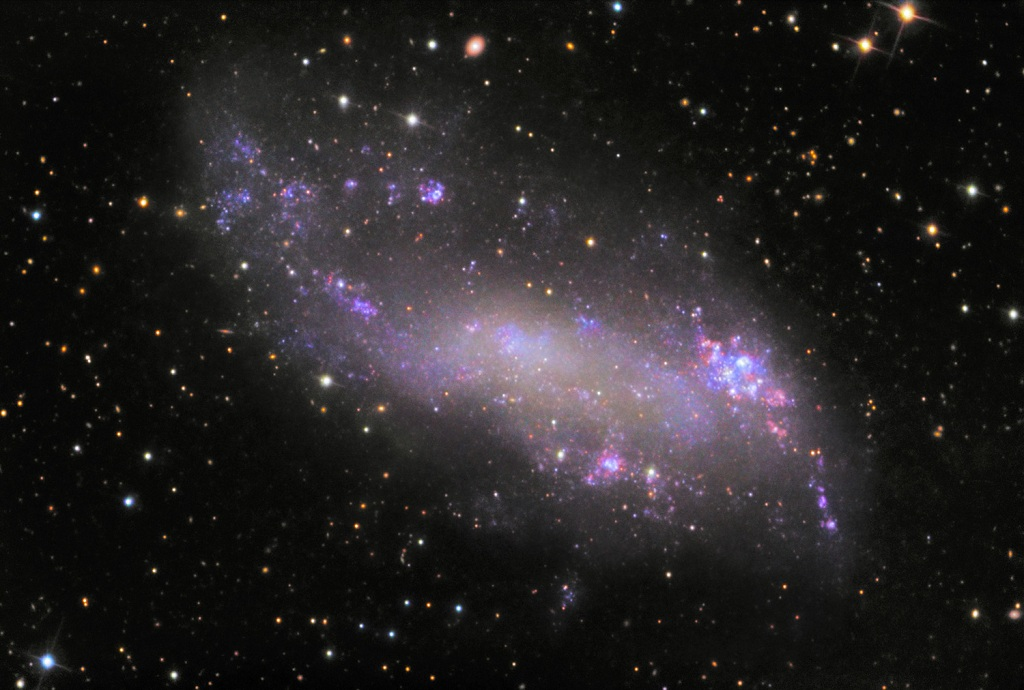
\includegraphics[width=\textwidth]{IC-2574.jpg}
                \newline
            \end{center}
        \end{column}

    \end{columns}

}

\frame
{
    \frametitle{Real Galaxies}

    \setbeamerfont*{itemize/enumerate body}{size=\Large}
    \setbeamerfont*{itemize/enumerate subbody}{parent=itemize/enumerate body}
    \setbeamerfont*{itemize/enumerate subsubbody}{parent=itemize/enumerate body}
 
    \begin{center}
        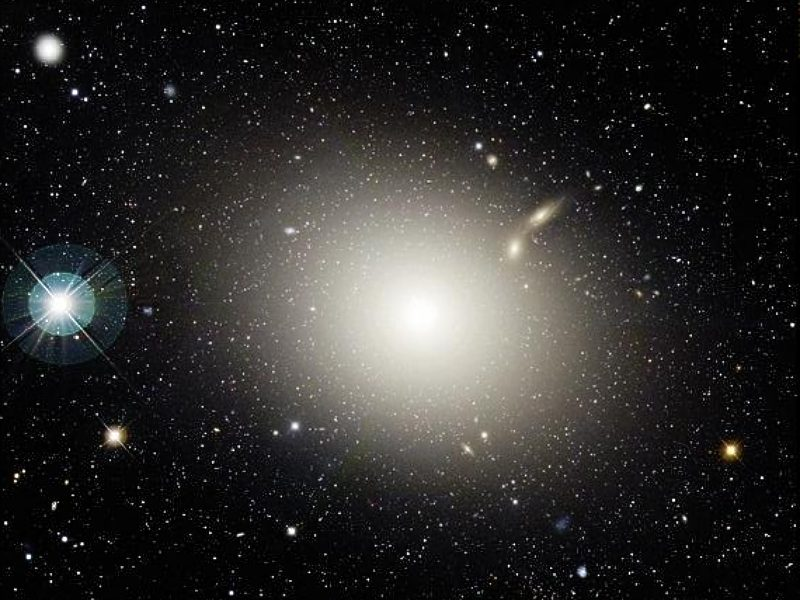
\includegraphics[width=\textwidth]{M87.jpg}
        \newline
    \end{center}

}

\frame
{
    \frametitle{Real Galaxies}

    \setbeamerfont*{itemize/enumerate body}{size=\Large}
    \setbeamerfont*{itemize/enumerate subbody}{parent=itemize/enumerate body}
    \setbeamerfont*{itemize/enumerate subsubbody}{parent=itemize/enumerate body}
 
    \begin{center}
        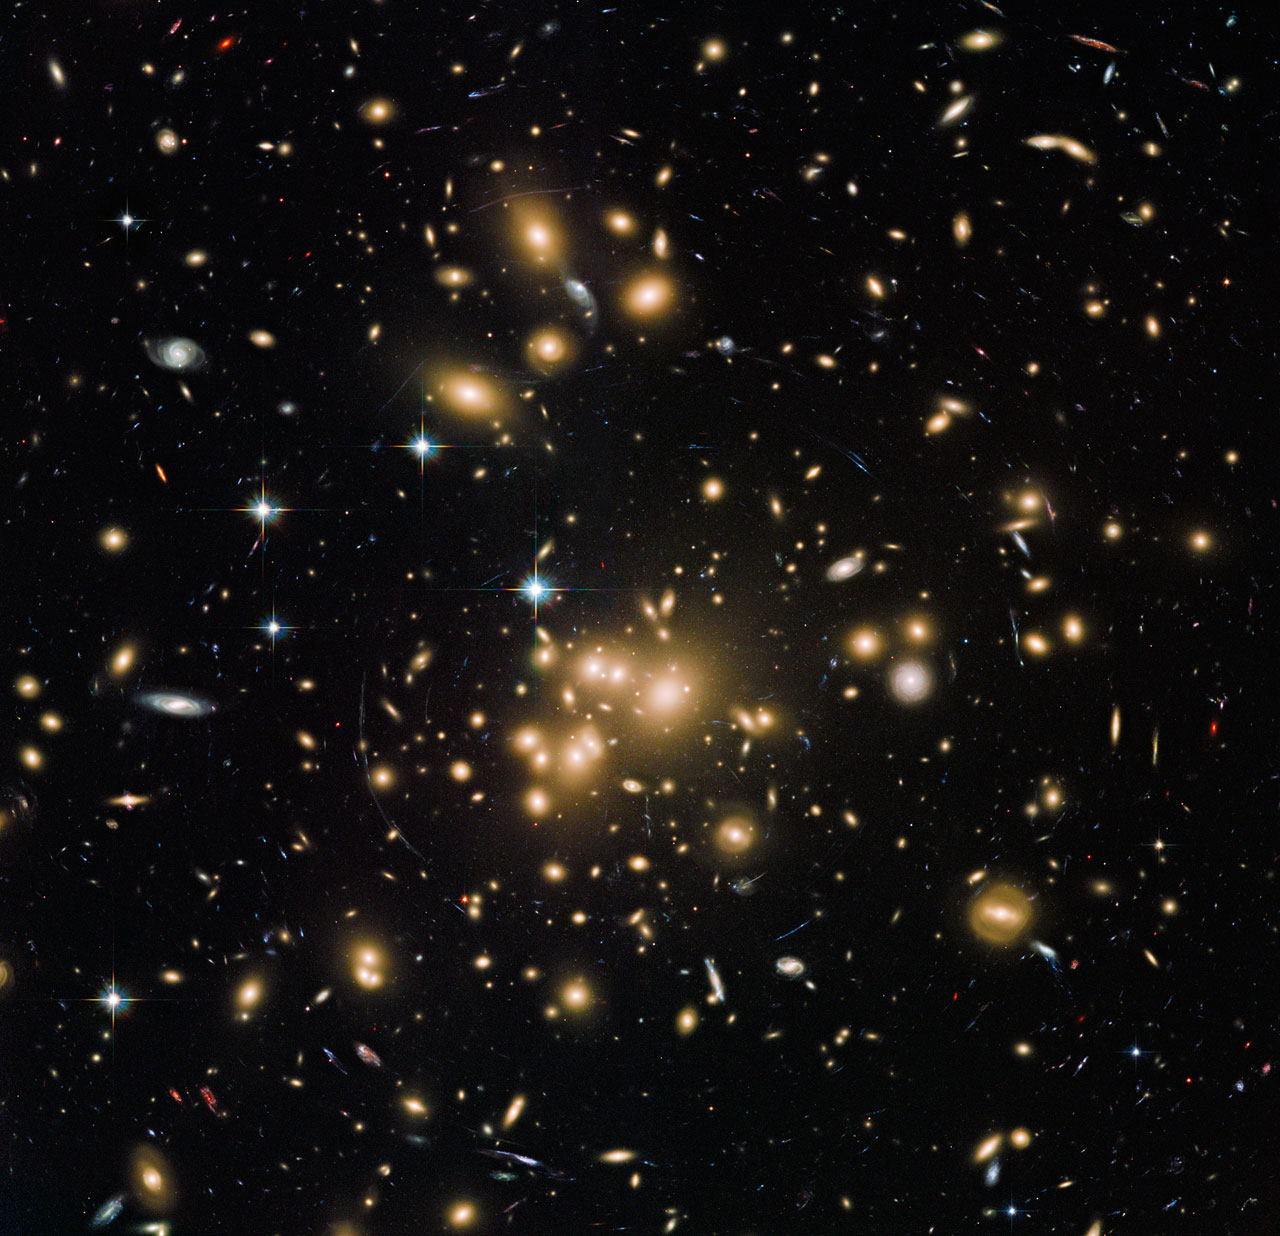
\includegraphics[width=0.75\textwidth]{heic1317a.jpg}
        \newline
    \end{center}

}

\frame
{
    \frametitle{Real Galaxies}

    \setbeamerfont*{itemize/enumerate body}{size=\Large}
    \setbeamerfont*{itemize/enumerate subbody}{parent=itemize/enumerate body}
    \setbeamerfont*{itemize/enumerate subsubbody}{parent=itemize/enumerate body}
 
    \begin{center}
        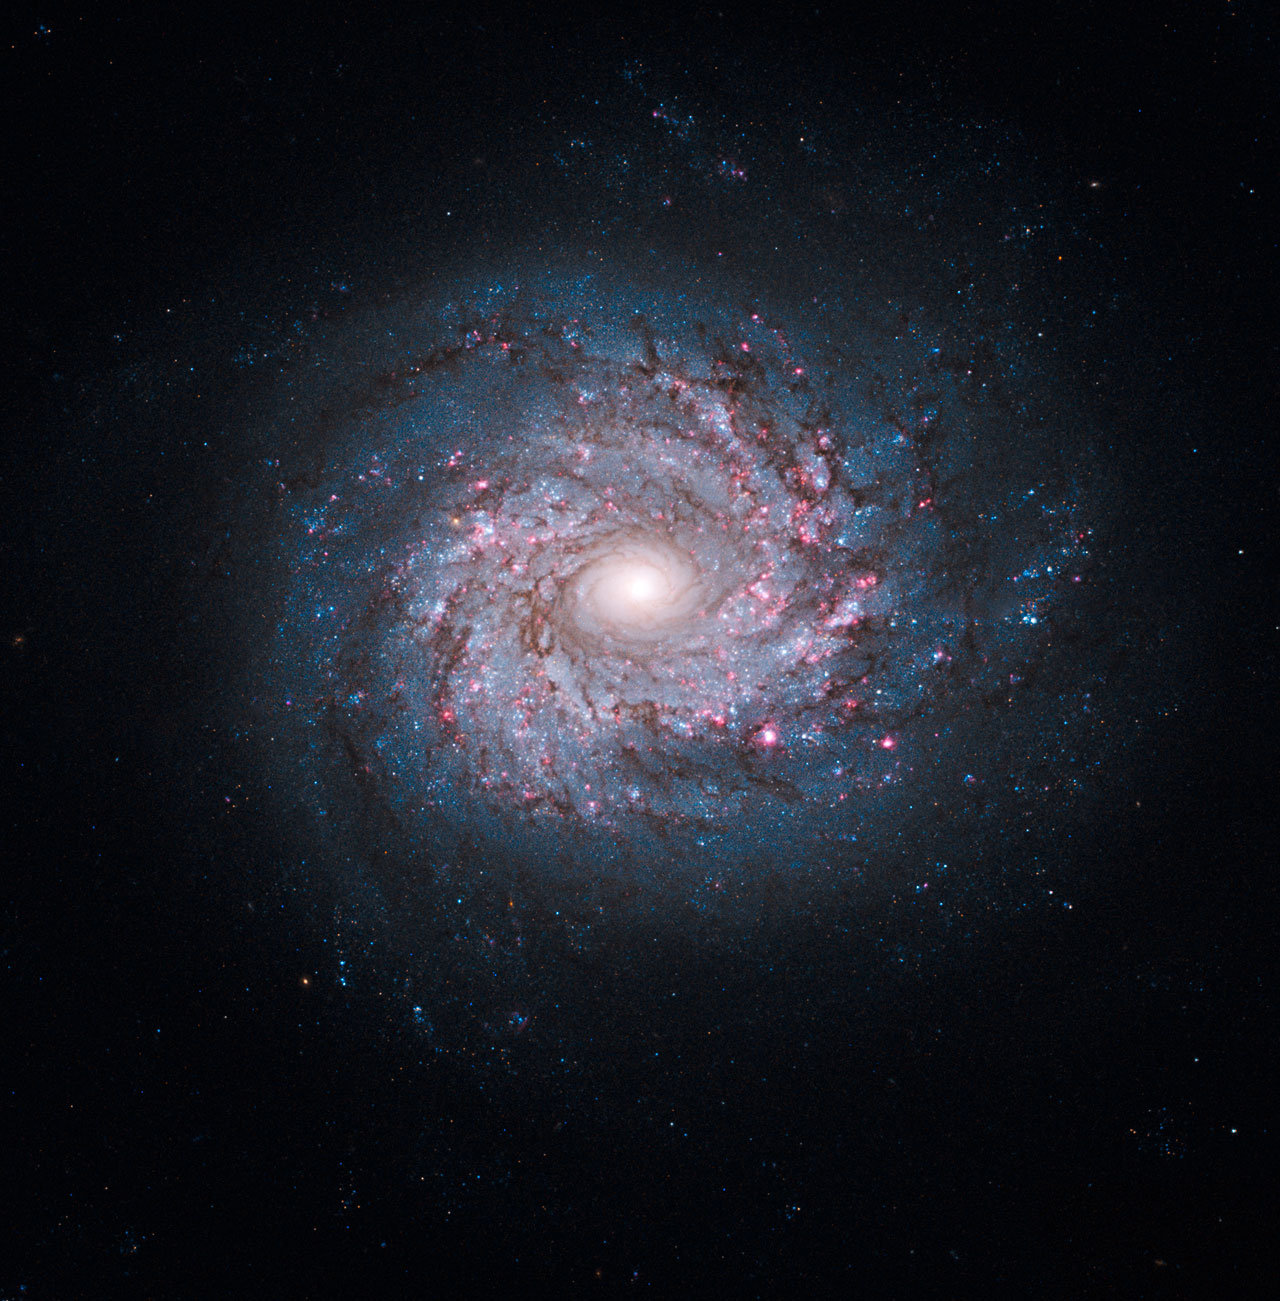
\includegraphics[width=0.8\textwidth]{opo1036a.jpg}
        \newline
    \end{center}

}



\frame
{
    \frametitle{Real Galaxies}

    \setbeamerfont*{itemize/enumerate body}{size=\Large}
    \setbeamerfont*{itemize/enumerate subbody}{parent=itemize/enumerate body}
    \setbeamerfont*{itemize/enumerate subsubbody}{parent=itemize/enumerate body}
 
    \begin{center}
        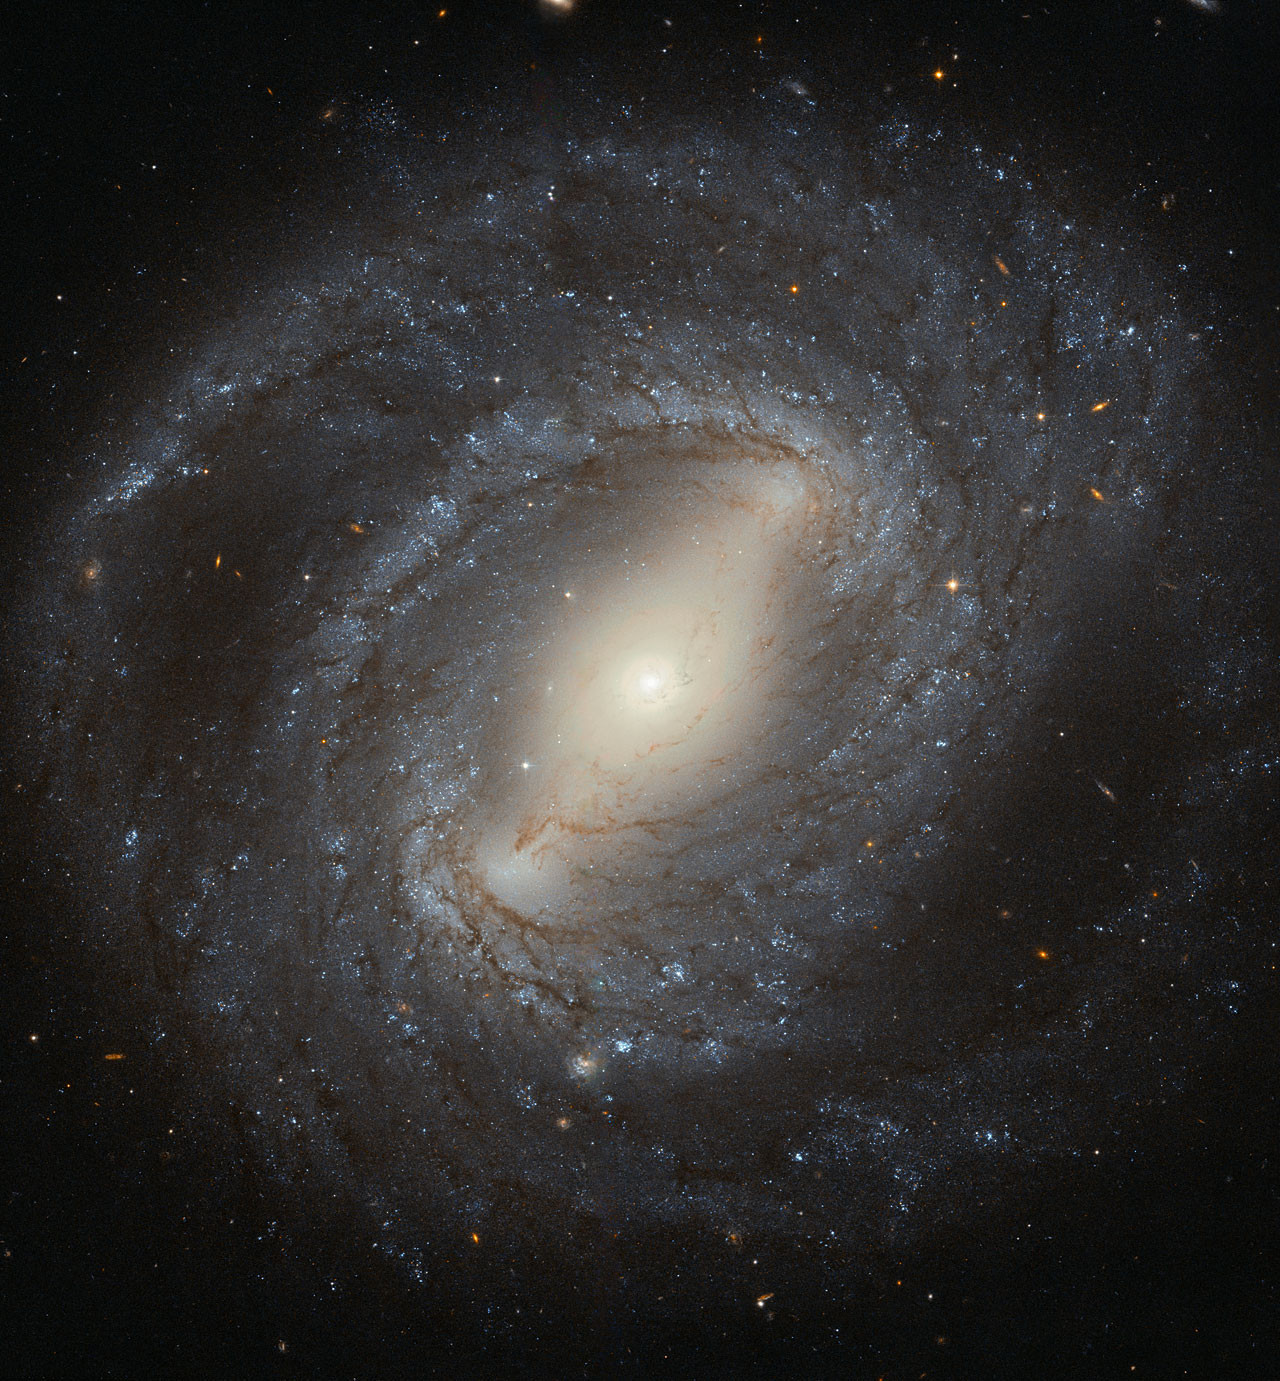
\includegraphics[width=0.7\textwidth]{NGC_4394_1280x1381.jpg}
        \newline
    \end{center}

}


\frame
{
    \frametitle{Real Galaxies}

    \setbeamerfont*{itemize/enumerate body}{size=\Large}
    \setbeamerfont*{itemize/enumerate subbody}{parent=itemize/enumerate body}
    \setbeamerfont*{itemize/enumerate subsubbody}{parent=itemize/enumerate body}
 
    \begin{center}
        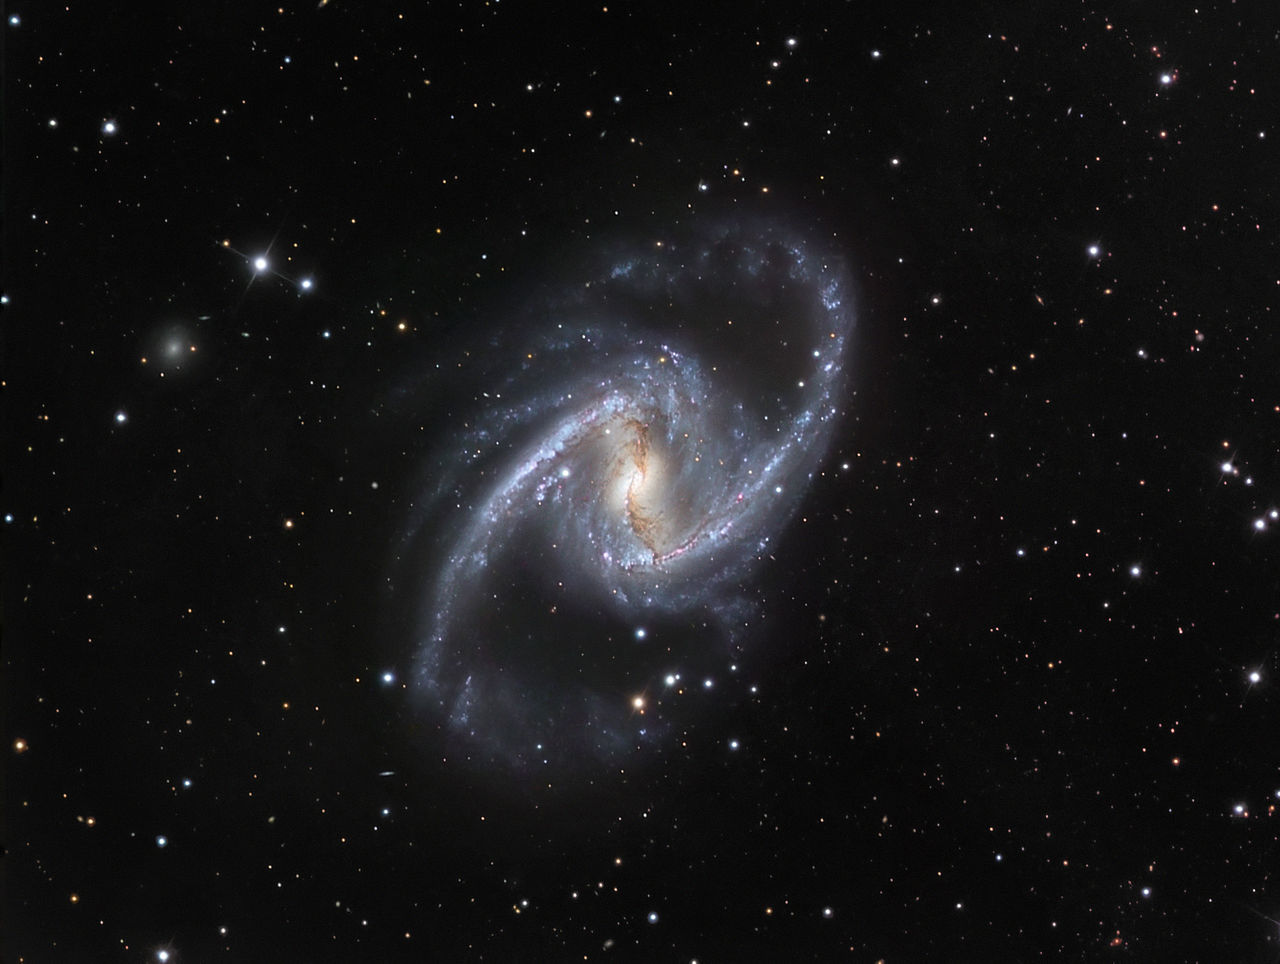
\includegraphics[width=0.75\textwidth]{NGC-1365-Great-Barred-Spiral-Galaxy.jpg}
        \newline
    \end{center}

}



\frame
{
    \frametitle{Real Galaxies}

    \setbeamerfont*{itemize/enumerate body}{size=\Large}
    \setbeamerfont*{itemize/enumerate subbody}{parent=itemize/enumerate body}
    \setbeamerfont*{itemize/enumerate subsubbody}{parent=itemize/enumerate body}
 
    \begin{center}
        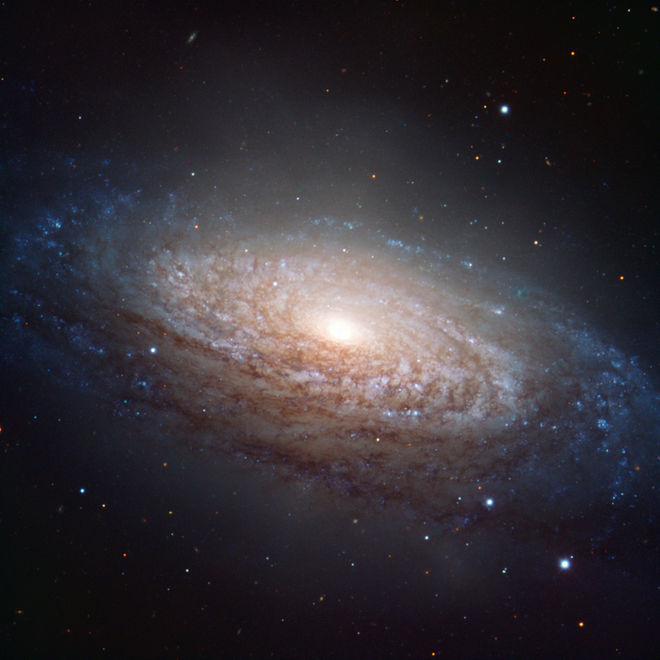
\includegraphics[width=0.75\textwidth]{spiral-galaxy-leo-constellation.jpg}
        \newline
    \end{center}

}




\frame
{
    \frametitle{Real Galaxies}

    \setbeamerfont*{itemize/enumerate body}{size=\Large}
    \setbeamerfont*{itemize/enumerate subbody}{parent=itemize/enumerate body}
    \setbeamerfont*{itemize/enumerate subsubbody}{parent=itemize/enumerate body}
 
    \begin{center}
        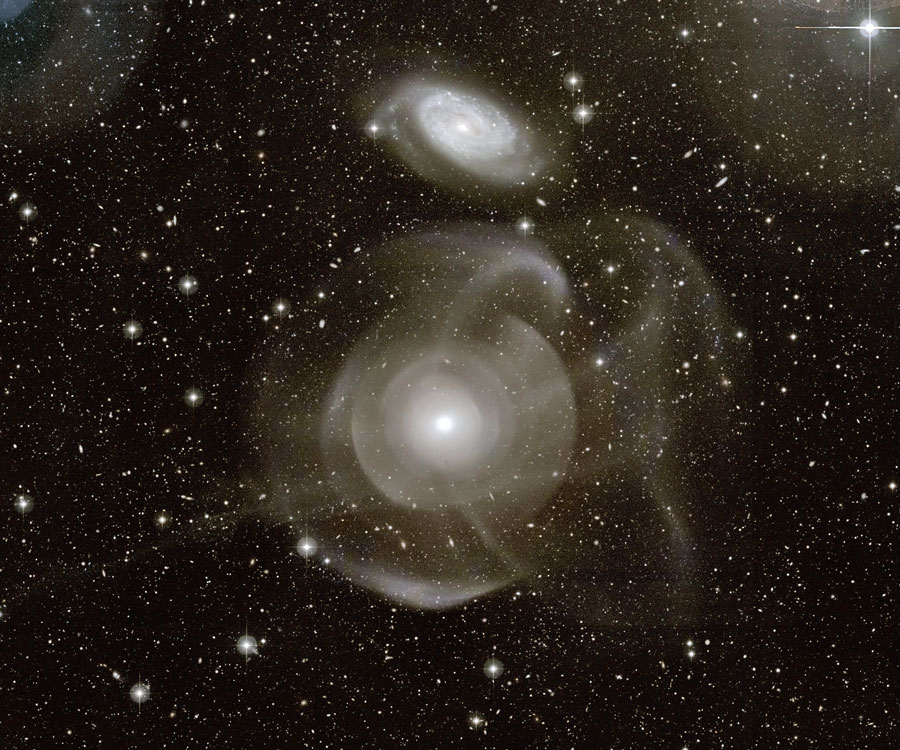
\includegraphics[width=\textwidth]{NGC474.png}
        \newline
    \end{center}

}


\frame
{
    \frametitle{Real Galaxies}

    \setbeamerfont*{itemize/enumerate body}{size=\Large}
    \setbeamerfont*{itemize/enumerate subbody}{parent=itemize/enumerate body}
    \setbeamerfont*{itemize/enumerate subsubbody}{parent=itemize/enumerate body}
 
    \begin{center}
        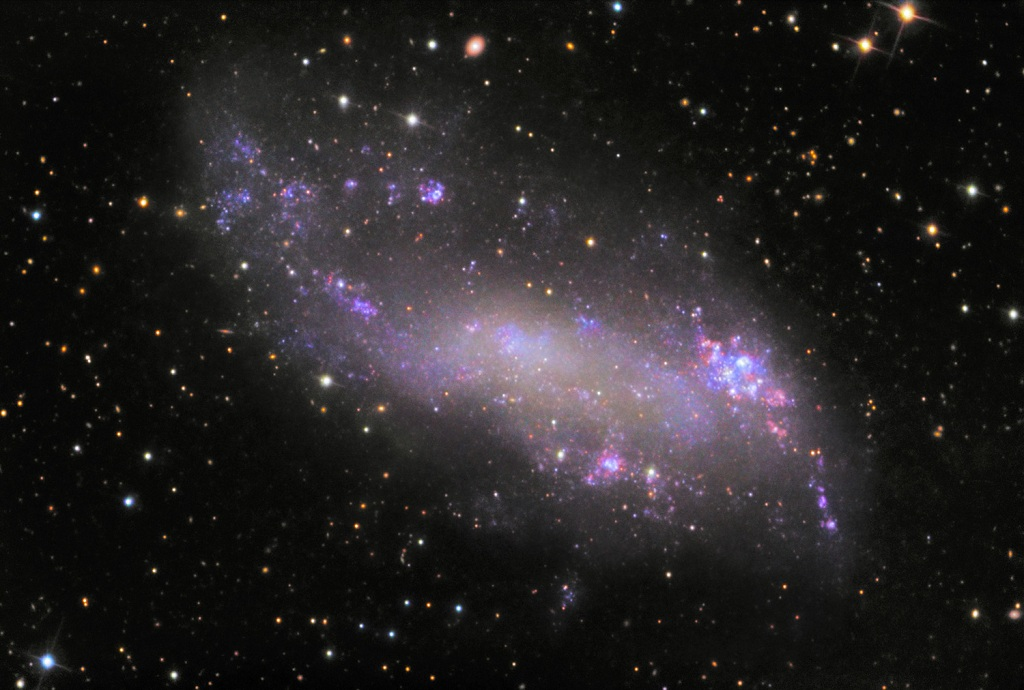
\includegraphics[width=\textwidth]{IC-2574.jpg}
        \newline
    \end{center}

}

\frame
{
    \frametitle{Real Galaxies}

    \setbeamerfont*{itemize/enumerate body}{size=\Large}
    \setbeamerfont*{itemize/enumerate subbody}{parent=itemize/enumerate body}
    \setbeamerfont*{itemize/enumerate subsubbody}{parent=itemize/enumerate body}
 
    \begin{center}
        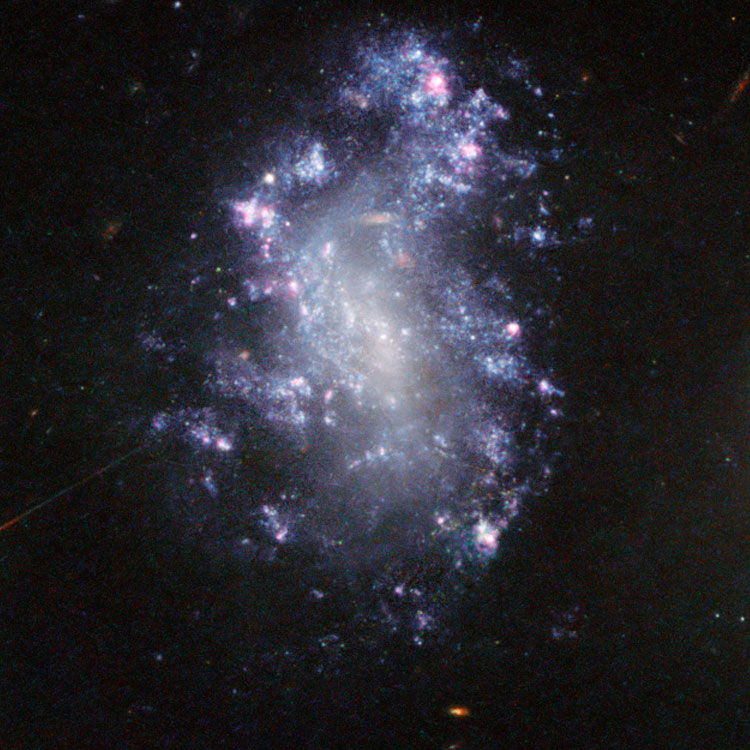
\includegraphics[width=0.7\textwidth]{pgc36867.jpg}
        \newline
    \end{center}

}


\frame
{
    \frametitle{Weak Lensing Model Bias}

    \setbeamerfont*{itemize/enumerate body}{size=\Large}
    \setbeamerfont*{itemize/enumerate subbody}{parent=itemize/enumerate body}
    \setbeamerfont*{itemize/enumerate subsubbody}{parent=itemize/enumerate body}
 
    \begin{columns}
        \begin{column}{0.5\textwidth}    


            \begin{itemize}

                \item Most shear measurement algorithms fit
                    some kind of simple elliptical model, and this
                    results in ``model bias''.

                \item Fitting more complex models is not possible: unstable

                \item With Metacalibration we can correct for
                    model bias.  We want to test this with
                    simulations.

            \end{itemize}
        \end{column}

        \begin{column}{0.5\textwidth}
            \begin{center}
                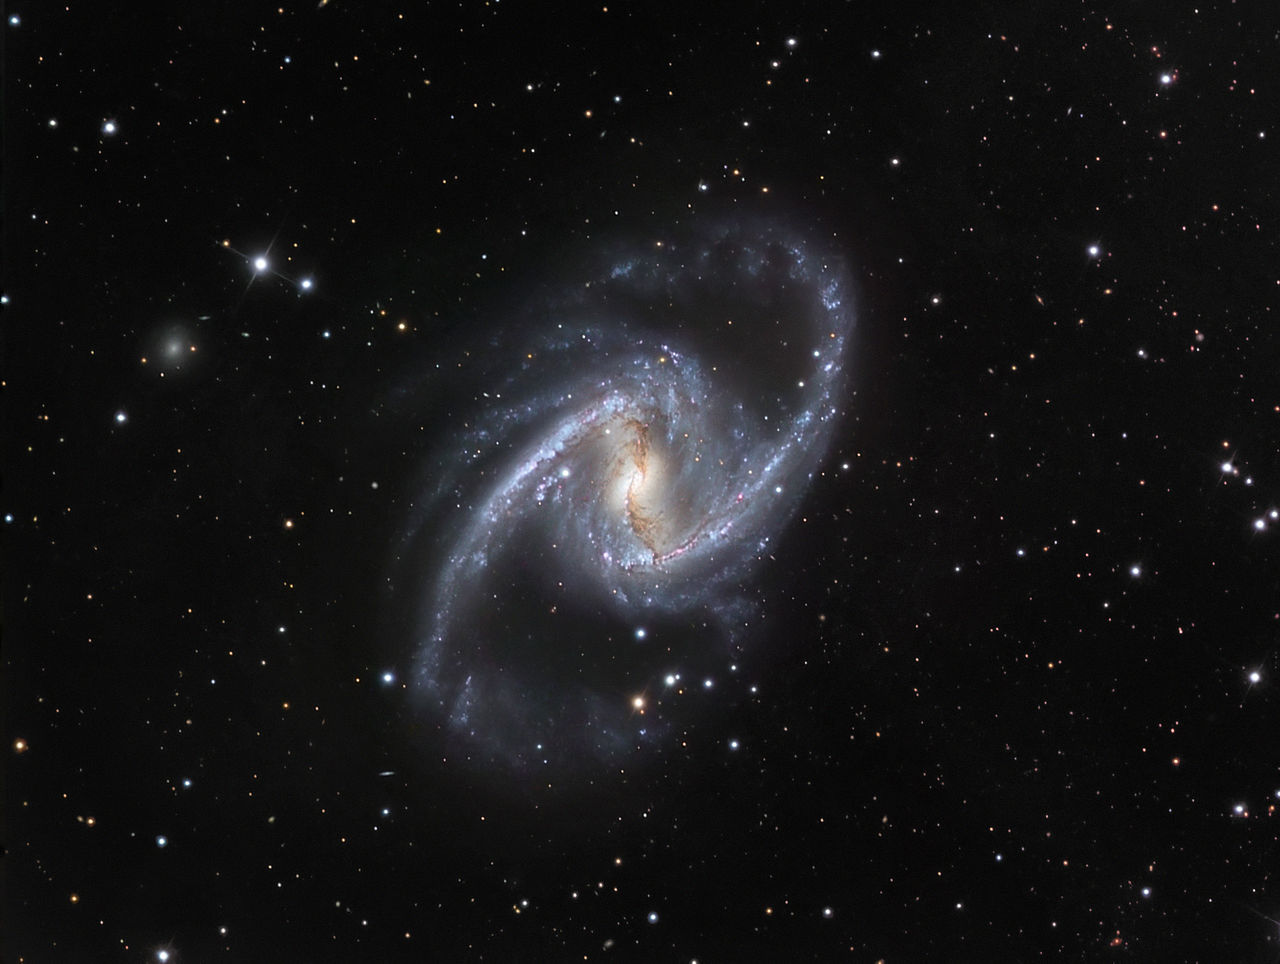
\includegraphics[width=0.75\textwidth]{NGC-1365-Great-Barred-Spiral-Galaxy.jpg}
                \newline
            \end{center}
        \end{column}

    \end{columns}

}

\frame
{
    \frametitle{Simulations}

    \setbeamerfont*{itemize/enumerate body}{size=\Large}
    \setbeamerfont*{itemize/enumerate subbody}{parent=itemize/enumerate body}
    \setbeamerfont*{itemize/enumerate subsubbody}{parent=itemize/enumerate body}
 
    \begin{itemize}
        \item Most common method to test model bias is to use HST images.
        \item Take real images, shear them, add extra noise, degrade psf
        \item This is very expensive
    \end{itemize}

}

\frame
{
    \frametitle{Alternate way: random walk}

    \setbeamerfont*{itemize/enumerate body}{size=\Large}
    \setbeamerfont*{itemize/enumerate subbody}{parent=itemize/enumerate body}
    \setbeamerfont*{itemize/enumerate subsubbody}{parent=itemize/enumerate body}
 
    \begin{itemize}
        \item Mentioned in Zhang et al. 2010 but with no details or code given;
            I implemented and added to Galsim

        \item Let a set of point sources take a ``random walk'' over the image

        \item Scale to requested scale radius and ellipticity

        \item Can represent an ``irregular`` galaxy, or can add to bulge+disk
            model to simulate knots of star formation.

    \end{itemize}

}

\frame
{
    \frametitle{Example Simulated Galaxies}

    \setbeamerfont*{itemize/enumerate body}{size=\Large}
    \setbeamerfont*{itemize/enumerate subbody}{parent=itemize/enumerate body}
    \setbeamerfont*{itemize/enumerate subsubbody}{parent=itemize/enumerate body}
 
    Mostly bulge-like
    \begin{center}
        \includegraphics[width=0.7\textwidth]{{rw-seed234-fdev-0.994-knotfrac-0.587}.png}
        \newline
    \end{center}

}

\frame
{
    \frametitle{Example Simulated Galaxies}

    \setbeamerfont*{itemize/enumerate body}{size=\Large}
    \setbeamerfont*{itemize/enumerate subbody}{parent=itemize/enumerate body}
    \setbeamerfont*{itemize/enumerate subsubbody}{parent=itemize/enumerate body}
 
    Mostly disk-like
    \begin{center}
        \includegraphics[width=0.7\textwidth]{{rw-seed234-fdev-0.024-knotfrac-0.025}.png}
        \newline
    \end{center}

}

\frame
{
    \frametitle{Example Simulated Galaxies}

    \setbeamerfont*{itemize/enumerate body}{size=\Large}
    \setbeamerfont*{itemize/enumerate subbody}{parent=itemize/enumerate body}
    \setbeamerfont*{itemize/enumerate subsubbody}{parent=itemize/enumerate body}
 
    disk-like with some knots of star formation
    \begin{center}
        \includegraphics[width=0.7\textwidth]{{rw-seed234-fdev-0.024-knotfrac-0.346}.png}
        \newline
    \end{center}

}

\frame
{
    \frametitle{Example Simulated Galaxies}

    \setbeamerfont*{itemize/enumerate body}{size=\Large}
    \setbeamerfont*{itemize/enumerate subbody}{parent=itemize/enumerate body}
    \setbeamerfont*{itemize/enumerate subsubbody}{parent=itemize/enumerate body}
 
    disk-like with more knots of star formation
    \begin{center}
        \includegraphics[width=0.7\textwidth]{{rw-seed234-fdev-0.028-knotfrac-0.549}.png}
        \newline
    \end{center}

}


\frame
{
    \frametitle{Example Simulated Galaxies}

    \setbeamerfont*{itemize/enumerate body}{size=\Large}
    \setbeamerfont*{itemize/enumerate subbody}{parent=itemize/enumerate body}
    \setbeamerfont*{itemize/enumerate subsubbody}{parent=itemize/enumerate body}
 
    mostly irregular
    \begin{center}
        \includegraphics[width=0.7\textwidth]{{rw-seed234-fdev-0.004-knotfrac-0.973}.png}
        \newline
    \end{center}

}



\frame
{
    \frametitle{Metacalibration}

    \setbeamerfont*{itemize/enumerate body}{size=\Large}
    \setbeamerfont*{itemize/enumerate subbody}{parent=itemize/enumerate body}
    \setbeamerfont*{itemize/enumerate subsubbody}{parent=itemize/enumerate body}
 
    \begin{itemize}
        \item I've been using these to test metacalibration
        \item Ten times faster than using HST images.
        \item So far metacal passes all tests.
    \end{itemize}

}






\end{document}
